% Compile with XeLaTeX (twice for cross-references), or Tectonic.
% Standalone CVPR-style course report: no cvpr.sty or .bib file required.
% This approximates CVPR typography; it is not an official submission template.
% Chinese names are retained exactly as supplied; all report prose is English.
% HW3: text added or changed since HW1 is blue (\new{...} or {\color{blue} ...}).
\documentclass[10pt,twocolumn,letterpaper]{article}
\usepackage[letterpaper,textwidth=6.875in,textheight=8.875in,top=1in,columnsep=0.3125in]{geometry}
\usepackage{fontspec}
\setmainfont{texgyretermes}[
  Extension=.otf,
  UprightFont=*-regular,
  BoldFont=*-bold,
  ItalicFont=*-italic,
  BoldItalicFont=*-bolditalic]
\usepackage{xeCJK}
% TeX Live's AR PL Mingti2L Big5 font supports Traditional Chinese names.
\setCJKmainfont{bsmi00lp.ttf}
% Report missing glyphs as errors rather than silently omitting names.
\tracinglostchars=3
\usepackage{amsmath,amssymb,booktabs}
\usepackage{graphicx}
\usepackage{xcolor}
% HW3: every figure/table caption is new, so label and text are blue.
\usepackage{caption}
\DeclareCaptionFont{blue}{\color{blue}}
\captionsetup{labelfont=blue,textfont=blue}
\usepackage{tikz}
\usetikzlibrary{arrows.meta,positioning}
\usepackage{titlesec}
\usepackage[hidelinks]{hyperref}
\hypersetup{pdftitle={Shaolin Duck Soccer: Autonomous Microduck Shooting with Hierarchical Reinforcement Learning}}
\graphicspath{{figures/}}
\newcommand{\new}[1]{{\color{blue}#1}}
\titleformat{\section}{\large\bfseries}{\thesection.}{0.5em}{}
\titleformat{\subsection}{\normalsize\bfseries}{\thesubsection.}{0.5em}{}
\titlespacing*{\section}{0pt}{9pt plus 2pt minus 1pt}{4pt}
\titlespacing*{\subsection}{0pt}{6pt plus 1pt minus 1pt}{3pt}
\setlength{\parindent}{1em}
\setlength{\parskip}{0pt}
\setlength{\emergencystretch}{1em}
\setlength{\abovedisplayskip}{5pt}
\setlength{\belowdisplayskip}{5pt}
\pagestyle{plain}
% HW1's two-page guard is removed: HW3 states no page limit.
\begin{document}
\twocolumn[{
\centering
{\fontsize{15}{17}\selectfont\bfseries Shaolin Duck Soccer: Autonomous Microduck Shooting\\
with Hierarchical Reinforcement Learning\par}
\vspace{9pt}
{\normalsize\bfseries Team Members\par}
\vspace{3pt}
{\normalsize
曾令城 (F74122030)\quad 黃威誠 (F74125313)\quad
葉沁蓉 (F74126238)\quad 李和穆 (E64112287)\par}
\vspace{3pt}
{\normalsize National Cheng Kung University\par}
\vspace{13pt}
}]

\begin{center}\bfseries Abstract\end{center}
\noindent\textit{We propose Shaolin Duck Soccer, a simulated bipedal robot that autonomously approaches a ball, aligns with a goal, and initiates a shot. A hierarchical controller will reuse fixed walking and kicking policies while a high-level policy, trained with Proximal Policy Optimization (PPO), selects movement commands and kick timing from simulator state. A curriculum will gradually expand initial distances, heading variations, and goal configurations. We will compare a geometric rule-based controller, high-level PPO without a curriculum, and PPO with a curriculum using identical low-level skills. Evaluation will measure valid goal rate, completion time, falls, and generalization. Deliverables include a reproducible simulation, autonomous shooting demonstrations, and a controlled analysis of skill composition and training schedules. Vision and hardware deployment are outside the core scope; two-robot passing is an optional extension.
\new{All three methods are now implemented and evaluated on 300 held-out episodes. The frozen skills are restrictive: the official kick scores only from a ball within about $\pm$2\,cm of its trained position, and the walking skill ignores commands below about 0.15\,m/s, which caps the geometric controller at 40.3\% valid goals. With the same skills, high-level PPO reaches 95.3\% without and 92.3\% with the curriculum (one training seed each) by commanding speeds above the walking dead zone and triggering the kick while still walking.}}

\section{Introduction}
Walking and kicking skills alone do not solve autonomous shooting. A robot must approach the ball from a suitable direction, establish a foot-specific stance, and switch skills without losing balance. Simply walking toward the ball can produce an inaccurate shot. Our central question is whether a learned high-level controller can coordinate existing skills more effectively across changing ball--goal configurations, and whether curriculum learning improves training efficiency.

Microduck provides an open platform for reusing locomotion and kicking policies~\cite{microduck}. Prior work studies transitions between primitive skills~\cite{lee}, agile bipedal soccer~\cite{haarnoja}, and directional striking under noisy sensing~\cite{xu}. SkillX investigates unified soccer skills~\cite{skillx}, while MARLadona addresses cooperative team play~\cite{marladona}. We target a smaller, reproducible task on Microduck rather than claim a new soccer capability: a single robot, an initially stationary ball, and an undefended goal on flat ground. Observations come from the simulator; camera perception, opponents, and physical deployment are excluded. The contribution will be the task implementation and a controlled comparison of decision strategies and training curricula.

{\color{blue}In the public Microduck stack, skills are switched by a human operator: a keyboard in the simulator rehearsal and a command on the robot. No learned high-level controller exists, so our goal is to replace that operator with a learned policy. Progress so far: (i) a soccer environment with a strict valid-shot detector; (ii) an adapter that runs the frozen ONNX skills batched on the GPU under a 10\,Hz high-level policy; (iii) measurements that quantify why the skills are hard to compose; and (iv) a first controlled comparison of methods A, B and C.\par}

\section{Method}
\subsection{Environment and Skill Reuse}
We will extend the official Microduck simulation with a goal, randomized episode initialization, termination conditions, and evaluation logging. Public ONNX policies will support initial skill validation. If parallel training requires compatible PyTorch checkpoints, we will obtain them or reproduce the required skills using the official training setup. All methods will share the same frozen low-level policies.

A valid goal requires the ball to cross the goal plane from the field into the opening between the posts. To distinguish shooting from continuous pushing, we will also record kick activation, kicking-foot contact, and subsequent ball separation. Falls, timeouts, and out-of-bounds events will terminate unsuccessful episodes.

{\color{blue}\textbf{Implemented scene.} The field is 2.0\,m$\times$1.2\,m with an undefended goal (0.40\,m wide, 0.20\,m crossbar) on the $+x$ boundary. Each episode places the ball 0.45--1.10\,m from the goal and $\pm$0.30\,m laterally; the robot starts 0.10--0.45\,m behind the right-foot preparation pose with $\pm$0.12\,m lateral and $\pm$90$^\circ$ heading offsets. Episodes last 12\,s. The robot keeps the repository's BAM servo model~\cite{bam} and domain randomization (mass, centre of mass, friction, armature, encoder bias, IMU misalignment, observation noise and delay). One hundred held-out layouts are generated once from a fixed seed (20261023) before any tuning.

\textbf{Valid shot.} A crossing counts only if the robot's \emph{last} touch of the ball was a kick: the kick skill was triggered, the right-foot collision geometry touched the ball while the kick skill owned the joints, and the ball then left the robot while moving. Any touch while walking voids the attempt, and each new kick starts a fresh one, so ``kick once, then walk the ball in'' never scores. Crossing is tested at the interpolated goal-plane intersection, so a fast ball cannot skip the detector. Testing the detector against the simulator exposed that MuJoCo's soft contact rests the ball centre 0.4\,mm below its radius, which made every rolling ball fail the original under-the-crossbar check; we allow 5\,mm of ground penetration and cover the case with a unit test.\par}

\subsection{Hierarchical Controller}
The high-level policy receives robot proprioception, robot-relative ball position and velocity, relative goal center and orientation, and the current skill and its progress. Its initial action interface is
\begin{equation}
 a_t^H=(v_x^{\mathrm{cmd}},v_y^{\mathrm{cmd}},\omega_z^{\mathrm{cmd}},z_{\mathrm{kick}}).
\end{equation}
The first three components command walking; a fixed threshold on the fourth triggers a kick, rather than setting kick strength. Shot direction is primarily determined by stance and heading. We will initially update the high-level policy at 10\,Hz and the low-level controller at 50\,Hz. A triggered kick will remain active for a validated duration to prevent rapid skill switching.

{\color{blue}\textbf{Frozen-skill adapter.} Fig.~\ref{fig:arch} shows the implemented stack. One high-level action drives five 50\,Hz steps of a frozen skill. While walking, the command is clamped to the walking policy's training ranges ($v_x\in[-0.4,0.4]$\,m/s, $v_y\in[-0.3,0.3]$\,m/s, $\omega_z\in[-1,1]$\,rad/s) and written into the twist slot of the shared 61-D low-level observation (48 proprioceptive dimensions and a 13-D command block). When $z_{\mathrm{kick}}>0$, the official right-foot kick takes over with an all-zero command for a 2\,s lockout that ignores further triggers. Both skills are the official ONNX files (pinned Hugging Face revision and SHA-256); because ONNX Runtime evaluates them one environment at a time, we re-implement their normalizer and MLP layers in PyTorch, which runs all 2048 environments in one GPU call and matches ONNX Runtime within $10^{-5}$. The high-level actor observes 48 dimensions (angular velocity, projected gravity, joint positions and velocities, ball position and velocity and goal centre and normal in the robot yaw frame, and the skill state); the critic additionally sees base linear velocity and the preparation-pose error (55-D).\par}

\begin{figure}[t]
\centering
\color{blue}
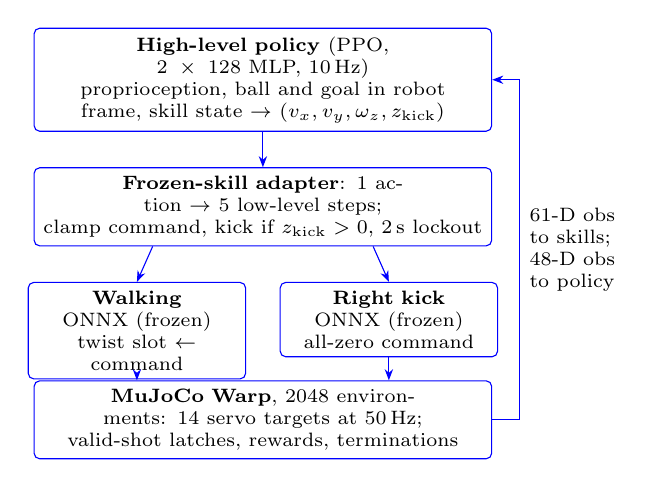
\begin{tikzpicture}[font=\scriptsize, node distance=4.5mm,
  box/.style={draw=blue, rounded corners=2pt, align=center, inner sep=3pt, text width=#1},
  arr/.style={-{Stealth[length=4pt]}, draw=blue}]
\node[box=5.6cm] (hl) {\textbf{High-level policy} (PPO, $2\times128$ MLP, 10\,Hz)\\
proprioception, ball and goal in robot frame, skill state $\rightarrow$ $(v_x, v_y, \omega_z, z_{\mathrm{kick}})$};
\node[box=5.6cm, below=of hl] (ad) {\textbf{Frozen-skill adapter}: 1 action $\rightarrow$ 5 low-level steps;\\
clamp command, kick if $z_{\mathrm{kick}}>0$, 2\,s lockout};
\node[box=2.55cm, below left=4.5mm and -2.7cm of ad] (walk) {\textbf{Walking} ONNX (frozen)\\twist slot $\leftarrow$ command};
\node[box=2.55cm, below right=4.5mm and -2.7cm of ad] (kick) {\textbf{Right kick} ONNX (frozen)\\all-zero command};
\node[box=5.6cm, below=17mm of ad] (sim) {\textbf{MuJoCo Warp}, 2048 environments: 14 servo targets at 50\,Hz;\\
valid-shot latches, rewards, terminations};
\draw[arr] (hl) -- (ad);
\draw[arr] (ad.south) ++(-1.4,0) -- (walk.north);
\draw[arr] (ad.south) ++(1.4,0) -- (kick.north);
\draw[arr] (walk.south) -- (walk.south |- sim.north);
\draw[arr] (kick.south) -- (kick.south |- sim.north);
\draw[arr] (sim.east) -- ++(0.35,0) |- node[pos=0.25, right, align=left] {61-D obs\\to skills;\\48-D obs\\to policy} (hl.east);
\end{tikzpicture}
\caption{\new{Implemented hierarchy. Only the high-level policy is trained.}}
\label{fig:arch}
\end{figure}

The geometric baseline will approach a foot-specific preparation pose, align with the goal, slow down, and trigger the same kick skill. For ball position $p_b$ and goal center $p_g$, define
\begin{equation}
 u_g=\frac{p_g-p_b}{\|p_g-p_b\|},\qquad
 p_r^*=p_b-R(\theta_g)r_{\mathrm{kick}},
\end{equation}
where $\theta_g$ is the heading of $u_g$, and $r_{\mathrm{kick}}$ is the calibrated ball offset for the selected kicking foot. This provides a meaningful baseline that accounts for shooting geometry.

{\color{blue}We use $r_{\mathrm{kick}}=(0.09,-0.042)$\,m, the kick's training ball position. The baseline commands $(v_x,v_y)=K\,(p_r^*-p_r)$ in the robot yaw frame and $\omega_z=K_\theta(\theta_g-\theta)$ with $K=K_\theta=2$, saturated at the walking ranges. Because the walking skill ignores small commands (Sec.~\ref{sec:deadzone}), a purely proportional approach stalls a few centimetres short of $p_r^*$; the baseline therefore kicks after position error, heading error ($<0.15$\,rad) and speed ($<0.05$\,m/s) have stayed within tolerance for 0.5\,s, and we sweep the position tolerance.\par}

\subsection{PPO and Curriculum}
We will train the high-level actor and critic with PPO~\cite{ppo}, initially using separate two-layer MLPs with 128 units per layer and normalized observations. Rewards will combine a once-per-episode valid-goal bonus, progress toward the preparation pose, improved alignment, and goal-directed ball motion after a valid kick, with penalties for falls, leaving the field, and elapsed time. Progress-based or bounded shaping will limit repeated reward collection without shooting. Both PPO variants will use identical rewards.

{\color{blue}The implemented reward per 50\,Hz step is
\begin{equation}
\begin{aligned}
r_t ={}& 10\,\mathbf{1}_{\mathrm{goal}} + 2\,\dot d_{\mathrm{prep}} + 0.5\,\dot e_{\theta}\\
 &+ 2\,\mathrm{clip}(v_{\mathrm{ball}}\!\cdot u_g,0,1.5)\,\mathbf{1}_{\mathrm{contact}}\\
 &- 0.5\,\mathbf{1}_{\mathrm{kick}} - 0.1 - 3\,\mathbf{1}_{\mathrm{fall}} - 2\,\mathbf{1}_{\mathrm{out}},
\end{aligned}
\end{equation}
where one-time terms are paid once per event and $\dot d_{\mathrm{prep}}$, $\dot e_\theta$ are the rates at which the distance to $p_r^*$ and the heading error decrease, paid only before the first kick. These two terms are potential-based~\cite{ng}: holding still earns nothing and moving away costs what moving back pays, so they cannot be farmed. The out-of-bounds penalty exceeds the time cost an early termination could save, so kicking the ball out never beats waiting. PPO uses learning rate $3\times10^{-4}$ with an adaptive KL schedule (target 0.01), clip 0.2, $\gamma=0.99$, $\lambda=0.95$, 5 epochs of 4 mini-batches, 24 high-level steps per environment per iteration, and initial action standard deviation 0.5.\par}

The curriculum will progress from near-ready shooting poses, to nearby starts with heading offsets, and finally to wider starting distances and varied goal configurations. Tentative distance ranges are 0.2--0.5\,m and 0.5--1.0\,m for the latter stages, subject to feasibility checks. Difficulty may increase when recent training success reaches 70\%, while retaining some easier episodes. These are initial design choices, not established optimal settings.

{\color{blue}\textbf{Implemented curriculum.} Stage~0 starts 0--5\,cm behind $p_r^*$ with $\pm$10$^\circ$ heading error and the ball 0.45--0.70\,m from the goal; stage~1 uses 5--25\,cm, $\pm$45$^\circ$ and 0.45--0.90\,m; stage~2 uses exactly method B's ranges, and both methods are evaluated on the same fixed layouts. We lowered the promotion gate to a 50\% goal rate over at least 2000 episodes and added a 300-iteration cap per stage, because method A reached only about 40\% with the same skills and a 70\% gate might never open. After promotion, 20\% of resets still draw from earlier stages. The stage is stored in checkpoints so an interrupted run resumes on the stage it reached.\par}

\subsection{Experimental Protocol}
We will compare the following methods:
\begin{center}
\small
\begin{tabular}{@{}cll@{}}
\toprule
 & High-level controller & Curriculum \\
\midrule
A & Geometry + state machine & -- \\
B & PPO & No \\
C & PPO & Yes \\
\bottomrule
\end{tabular}
\end{center}
Methods B and C will share network size, rewards, and total environment interaction budgets, including all curriculum stages. Method B will sample the full training distribution from the outset. All three methods will use identical skills and held-out test configurations. We target at least three training seeds and 100 evaluation episodes per final policy per condition. Test configurations will be fixed before tuning. We plan to use two borrowed RTX 4090 GPUs for independent runs after single-GPU validation.

{\color{blue}In practice, B and C use 2048 environments $\times$ 24 steps $\times$ 2000 iterations (98.3\,M high-level transitions), and every final policy is evaluated on the 100 held-out layouts three times (300 episodes, evaluation seed 0). Runs so far used two laptop GPUs (RTX 4050 6\,GB and RTX 4060 8\,GB) at about 9\,s per iteration.\par}

\section{\new{Experiments}}
\noindent\new{HW1's evaluation plan, kept below as the protocol, is followed by the results to date.}

\subsection{\new{Evaluation Protocol (from HW1)}}
We expect to deliver a system demonstrating approach, alignment, and shooting from frontal, lateral, and reversed-heading starts, including changed goal locations. Achieving at least 70\% valid goals over 100 standard test episodes is an engineering acceptance target, not a measured result or guaranteed prediction.

The primary metric will be valid goal rate over \emph{all} episodes, including falls, timeouts, and missed contacts. We will report successful-episode completion time separately from timeout frequency, along with fall rate, post-contact shot-direction error, and goal rate under held-out poses and mild physical variations. Episodes without a valid kick will remain failures. Learning efficiency will be measured in environment interactions needed to reach a specified success rate.

Results will include goal-rate learning curves with variation across seeds, spatial success maps, and matched trajectory and failure-case comparisons. We will test whether curricula improve convergence speed or final performance without assuming PPO must outperform geometry. Failures caused by low-level skills will be distinguished from high-level decision errors. Deliverables will include code, models, configurations, evaluation procedures, and success/failure videos. Fixed-target passing and, subsequently, two robots sharing one physical simulation are stretch goals informed by cooperative soccer research~\cite{marladona}.

{\color{blue}
\subsection{Setup}
All experiments run in simulation with mjlab 1.3.0~\cite{mjlab} (MuJoCo 3.10, MuJoCo Warp 3.8.1, Warp 1.12), rsl\_rl 5.0.1~\cite{rslrl} and PyTorch 2.9.1 with Python 3.12, on laptop RTX 4050 and RTX 4060 GPUs. Skill files are verified by SHA-256 on every machine, and the shared held-out layout file has the same SHA-256 on both.

\subsection{Reproducing the Low-Level Skills}
To validate the platform we first retrained the official recipes. The walking policy (2048 environments, 16.6k iterations, 7.8\,h) reached a mean episode length of 942 of 1000 steps with 0.25 falls per iteration, and the right-foot kick (2000 iterations, 67\,min) fell in about 1\% of episodes. Both behave like the official policies in the CPU deployment rehearsal. The soccer experiments nevertheless use the official files, so that results reflect the public skills.

\subsection{Blind-Kick Placement Tolerance}
The official kick does not observe the ball; it was trained with the ball at $r_{\mathrm{kick}}\pm1.5$\,cm. We placed the ball on a grid of offsets (forward $-1.5$ to $+7.5$\,cm, lateral $\pm$6\,cm, 1.5\,cm spacing, 32 kicks per cell, 2016 parallel environments) and scored crossings of a 0.30\,m goal 1\,m ahead (Fig.~\ref{fig:tolerance}). At the trained position it scores 53\%; beyond about $\pm$2\,cm laterally or $+3$\,cm forward it almost never scores because the foot misses the ball. Even well-placed kicks deviate $8.2^\circ\pm6.3^\circ$ to the right. The kick's reward pays only the forward component of ball velocity, capped at 1\,m/s, so its direction is unconstrained.

\begin{figure}[t]
\centering
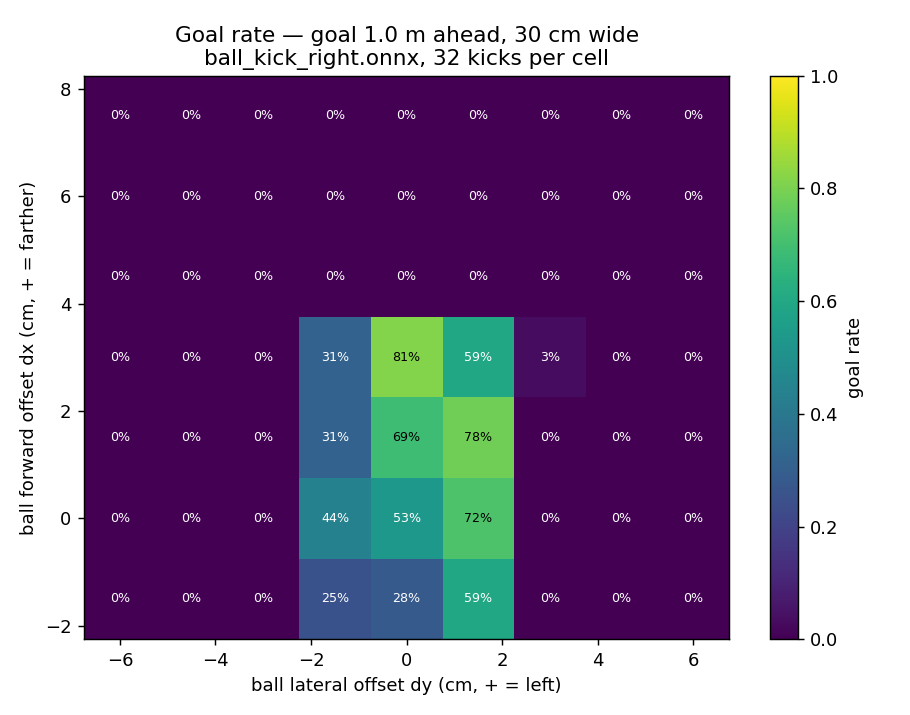
\includegraphics[width=0.92\columnwidth]{blind_kick_tolerance_official.png}
\caption{Goal rate of the official blind kick versus ball placement error (32 kicks per cell).}
\label{fig:tolerance}
\end{figure}

\subsection{Walking Dead Zone}\label{sec:deadzone}
Commanding the walking skill straight ahead gives these steady-state speeds, identical in its own training environment and in ours:
\begin{center}
\small
\begin{tabular}{@{}ccc@{}}
\toprule
command $v_x$ & velocity env & soccer env \\
\midrule
0.1\,m/s & 0.00\,m/s & 0.00\,m/s \\
0.2\,m/s & 0.03\,m/s & 0.06\,m/s \\
0.3\,m/s & 0.14\,m/s & 0.15\,m/s \\
\bottomrule
\end{tabular}
\end{center}
The skill therefore cannot make the centimetre-scale corrections the blind kick requires.

\subsection{Method A}
Fig.~\ref{fig:sweep} sweeps the baseline's kick tolerance over the held-out layouts (300 episodes per point). With the 2\,cm tolerance the kick needs, 87\% of episodes time out: the robot stalls a median 2.5\,cm from $p_r^*$. Relaxing the tolerance lifts the goal rate to a plateau of about 40\% (41.3\% at 6\,cm), because the robot stops about 3\,cm from $p_r^*$ regardless and the foot then touches the ball in only about two thirds of kicks. We use 5\,cm (40.3\%) below. Before the ground-penetration fix in the goal detector, the same baseline scored 1\%, which shows why the detector itself was tested.

\begin{figure}[t]
\centering
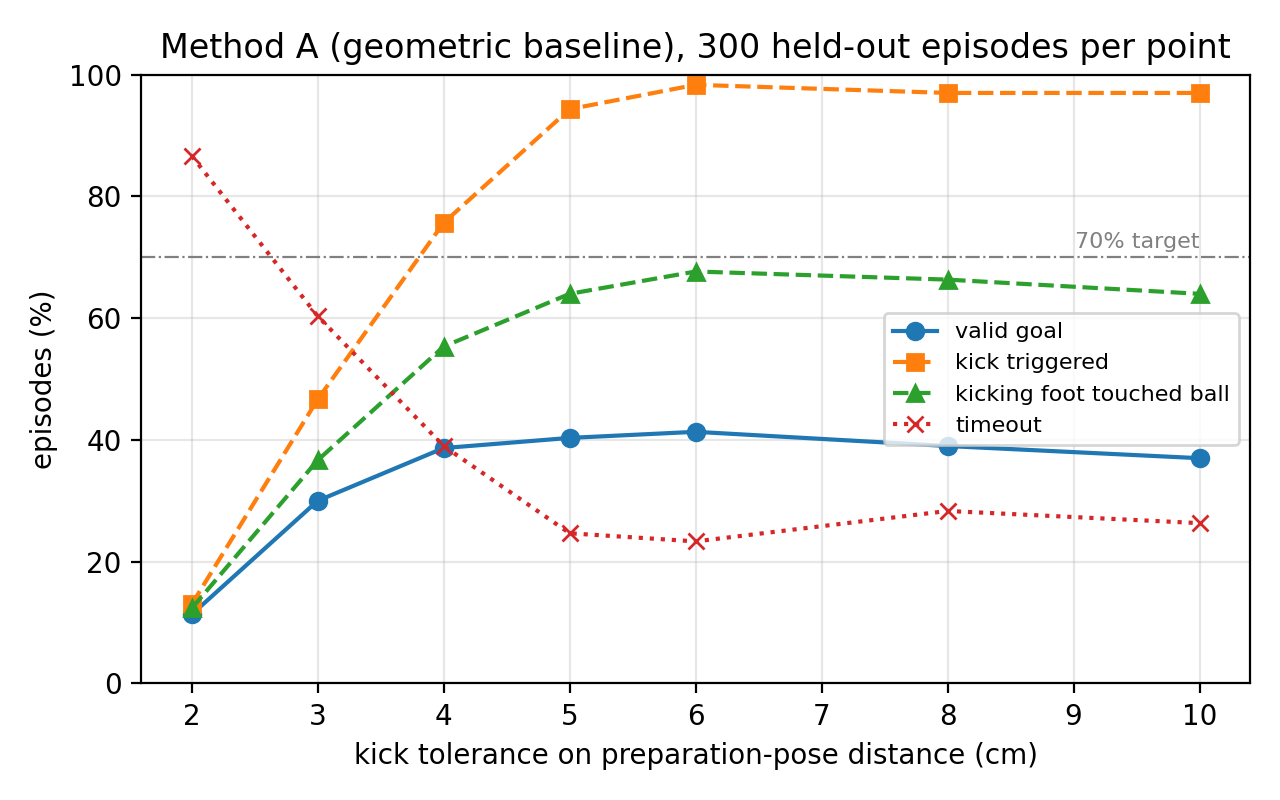
\includegraphics[width=\columnwidth]{baseline_kick_tolerance_sweep.png}
\caption{Method A versus its kick tolerance; 300 held-out episodes per point.}
\label{fig:sweep}
\end{figure}

\subsection{Methods B and C}
Table~\ref{tab:main} and Fig.~\ref{fig:abc} compare the three methods on the same 300 held-out episodes. B and C share commit, skills (identical SHA-256), budget and seed; their configurations differ only in C's curriculum term. Both PPO controllers exceed the 70\% target with the official skills. C evaluated on its own machine scored 94.0\%; on the same machine as B it scored 92.3\%. With only one trained seed per method, the 3-point same-machine B--C gap is descriptive: it does not estimate seed-to-seed training variance and therefore cannot support an algorithm-level claim that B outperforms C. The three evaluation repeats re-test one trained policy rather than provide additional training seeds.

\begin{table*}[t]
\centering
\small
\color{blue}
\begin{tabular}{@{}lcccccccc@{}}
\toprule
method & valid goal & foot contact & ball out & robot out & timeout & fell & goal time & error at kick \\
\midrule
A: geometric (5\,cm) & 40.3\% & 65.7\% & 31.7\% & 1.0\% & 26.7\% & 0.3\% & 4.9\,s & 3.0\,cm \\
B: PPO, seed 1 & \textbf{95.3\%} & 98.7\% & 2.3\% & 1.3\% & 0.3\% & 0.7\% & 3.2\,s & 1.4\,cm \\
C: PPO + curriculum, seed 1 & 92.3\% & 97.0\% & 5.3\% & 1.0\% & 0.3\% & 1.0\% & 3.3\,s & 2.3\,cm \\
\bottomrule
\end{tabular}
\caption{Results on the 100 held-out layouts $\times$ 3 repeats (300 episodes), all evaluated on the same machine. Rates are over all episodes; goal time is the mean over scoring episodes; error at kick is the median distance to $p_r^*$ when the kick is triggered.}
\label{tab:main}
\end{table*}

\begin{figure}[t]
\centering
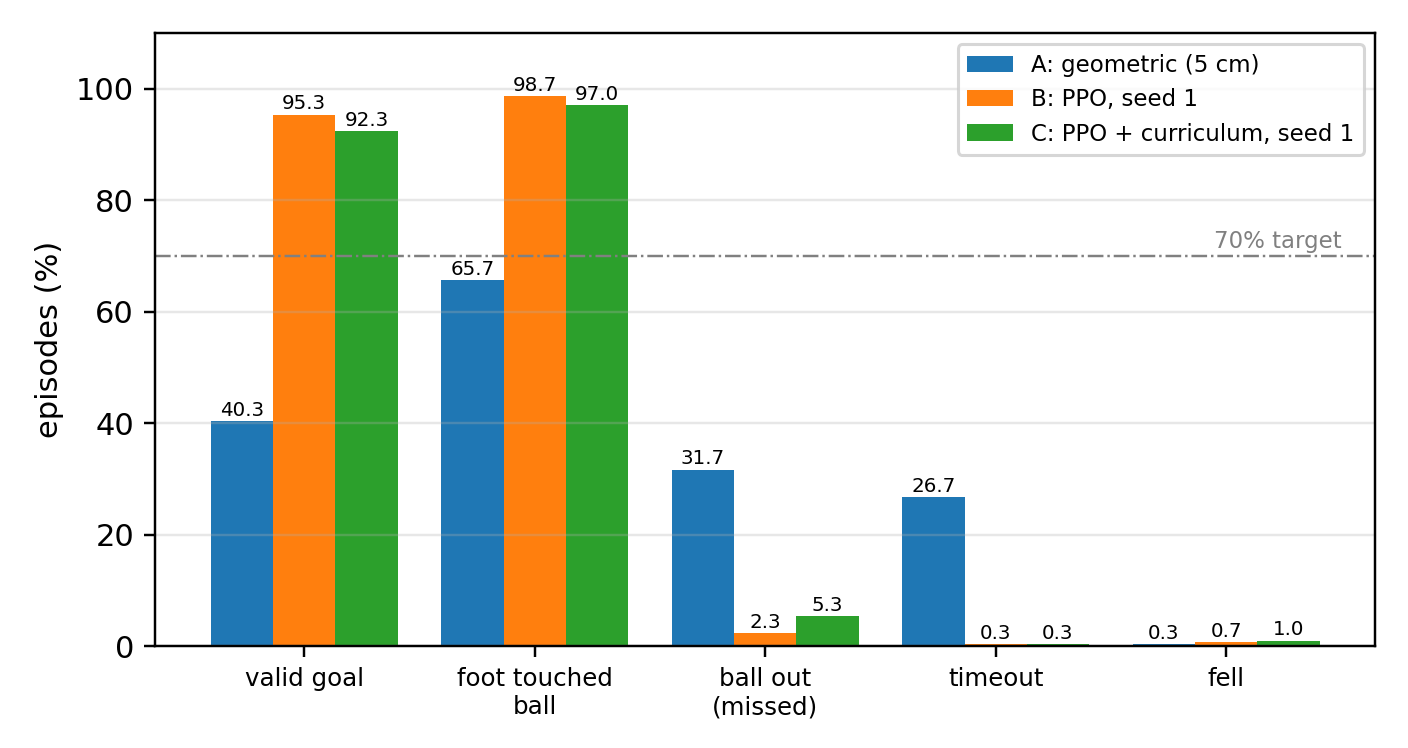
\includegraphics[width=\columnwidth]{methods_ABC.png}
\caption{Outcomes of methods A, B and C with identical frozen skills.}
\label{fig:abc}
\end{figure}

\textbf{How the learned controllers use the same skills.} Within 5\,cm of $p_r^*$, 96\% (B) and 99\% (C) of the commanded speeds exceed the walking dead zone (medians 0.31 and 0.50\,m/s), whereas none of method A's do (median 0.07\,m/s). Both trigger the kick while still walking (median robot speed 0.20 and 0.16\,m/s versus 0.001\,m/s for A), letting walking momentum carry the foot into place, which method A excludes by design. At the kick, B faces $3.1^\circ\pm3.7^\circ$ and C $7.8^\circ\pm5.7^\circ$ left of the shot line; C's aim nearly cancels the kick's $8.2^\circ$ right bias. Both kick about once per episode and score through foot contact, so the gains do not come from repeated attempts or pushing; videos confirm real shots.

\textbf{Training dynamics.} Mean episode length (10\,Hz steps; 120 is a timeout):
\begin{center}
\small
\begin{tabular}{@{}lccccc@{}}
\toprule
iteration & 25 & 50 & 100 & 150 & 200 \\
\midrule
B & 119 & 120 & 120 & 87 & 43 \\
C & 81 & 64 & 35 & 27 & 37 \\
\bottomrule
\end{tabular}
\end{center}
B first collapsed to never kicking (nearly every episode timed out from about iteration 5 to 140) because the kick-attempt cost was active from the start, and its mean reward turned positive only around iteration 150. C never collapsed: early kicks score on the near-ready stage, and its mean reward was positive by iteration 75. This is the early-exploration benefit the plan predicted, observed once. C's curriculum promoted at iterations 15 and 174, both by the 50\% gate, so C spent about 91\% of its training iterations in stage~2; even there, 20\% of resets still drew from the easier stages, so C never trained on exactly B's distribution.

\textbf{Fixed-test learning curves.} We also evaluated the checkpoints saved every 100 iterations (21 per method) on the same 300 held-out episodes (Fig.~\ref{fig:curve}; one RTX 4060, a separate batch from Table~\ref{tab:main}). After 101 updates C already scored 38.7\% while B scored 0\%, but B first reached 90\% at checkpoint 200 (92.7\%) and C only at 400 (94.3\%). From checkpoint 200 on, B scored at least as high as C at every checkpoint, ending at 95.7\% versus 94.0\%. In this single seed the curriculum sped up early learning but did not reach a high goal rate sooner. With checkpoints 100 iterations apart these are first observed crossings, not exact convergence times; checkpoints 0--200 were also evaluated with weaker centre-of-mass randomization than later ones, identically for B and C.

\begin{figure}[t]
\centering
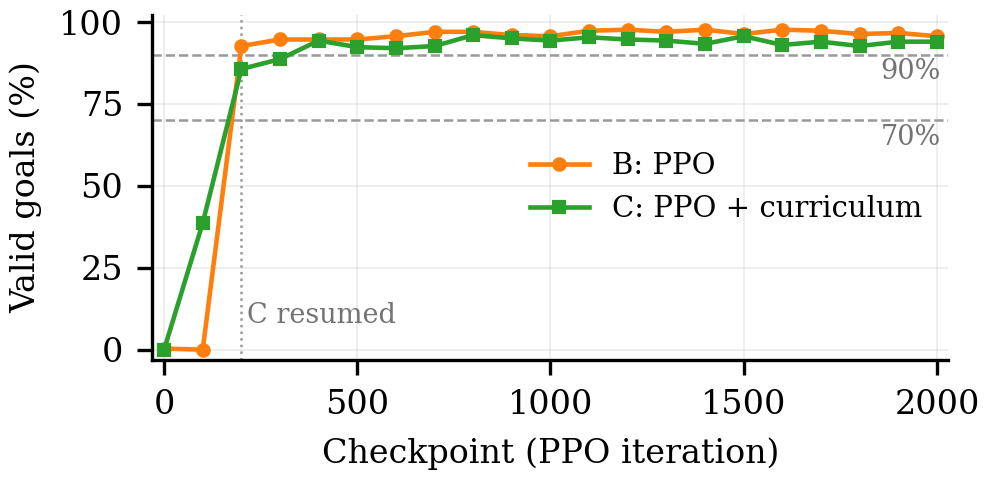
\includegraphics[width=\columnwidth]{learning_speed_seed1.png}
\caption{\new{Valid goal rate of every saved checkpoint on the 300 held-out episodes (training seed 1, RTX 4060). C was resumed from checkpoint 200 after a driver update.}}
\label{fig:curve}
\end{figure}

\subsection{Limitations and Next Steps}
Each learned method has one training seed so far. C's run was interrupted by a GPU driver update and resumed from iteration 200 (iterations 201--267 recomputed); its curriculum stage, not yet checkpointed at that commit, was restored from the log. Kicking on the move succeeds in simulation although the kick was trained from a standing start; we make no hardware claim. Next we will run seeds 2 and 3 for B and C, repeat the checkpoint evaluation on them, and build spatial success maps over start positions. Because B and C already exceed the target with the official skills, retraining the kick is no longer needed for the core comparison and becomes an extension.
\par}

\begin{thebibliography}{11}
\small
\setlength{\itemsep}{1pt}
\setlength{\parskip}{0pt}
\bibitem{microduck}
Pollen Robotics. \href{https://github.com/pollen-robotics/microduck_rl}{Microduck RL: RL training environments for Microduck}. Open-source software, accessed Sept.\ 29, 2026.
\bibitem{ppo}
J.~Schulman, F.~Wolski, P.~Dhariwal, A.~Radford, and O.~Klimov. \href{https://arxiv.org/abs/1707.06347}{Proximal policy optimization algorithms}. arXiv:1707.06347, 2017.
\bibitem{lee}
Y.~Lee, S.-H.~Sun, S.~Somasundaram, E.~S.~Hu, and J.~J.~Lim. \href{https://youngwoon.github.io/transition/}{Composing complex skills by learning transition policies}. In \emph{ICLR}, 2019.
\bibitem{haarnoja}
T.~Haarnoja et~al. \href{https://doi.org/10.1126/scirobotics.adi8022}{Learning agile soccer skills for a bipedal robot with deep reinforcement learning}. \emph{Science Robotics}, 2024.
\bibitem{xu}
Z.~Xu et~al. \href{https://arxiv.org/abs/2512.06571}{Learning agile striker skills for humanoid soccer robots from noisy sensory input}. In \emph{ICRA}, 2026. arXiv:2512.06571.
\bibitem{skillx}
Z.~Ye et~al. \href{https://arxiv.org/abs/2609.06718}{SkillX: Unified multi-skill policy learning for humanoid soccer}. arXiv:2609.06718, 2026.
\bibitem{marladona}
Z.~Li, F.~Bjelonic, V.~Klemm, and M.~Hutter. \href{https://arxiv.org/abs/2409.20326}{MARLadona---Towards cooperative team play using multi-agent reinforcement learning}. arXiv:2409.20326, 2024; revised 2025.
{\color{blue}
\bibitem{ng}
A.~Y.~Ng, D.~Harada, and S.~Russell. Policy invariance under reward transformations: Theory and application to reward shaping. In \emph{ICML}, 1999.
\bibitem{mjlab}
\href{https://github.com/mujocolab/mjlab}{mjlab: GPU-accelerated robot learning on MuJoCo Warp}. Open-source software, version 1.3.0.
\bibitem{rslrl}
\href{https://github.com/leggedrobotics/rsl_rl}{RSL-RL: Reinforcement learning library for robotics}. Open-source software, version 5.0.1.
\bibitem{bam}
Rhoban. \href{https://github.com/Rhoban/bam}{BAM: Better actuator models}. Open-source software.
}
\end{thebibliography}
\end{document}
